\begin{figure}[H]
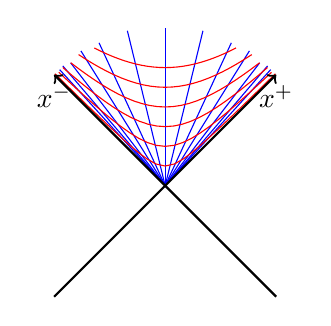
\begin{tikzpicture}
%\eta rapidity
\draw[color=blue] (0,0) -- (0,2); %0
\draw[color=blue][domain=-0.48:0.48] plot (\x,{4.1*abs(\x)}); %0.25
\draw[color=blue][domain=-0.84:0.84] plot (\x,{2.16*abs(\x)}); %0.5
\draw[color=blue][domain=-1.07:1.07] plot (\x,{1.6*abs(\x)}); %0.75
\draw[color=blue][domain=-1.2:1.2] plot (\x,{1.3*abs(\x)}); %1
\draw[color=blue][domain=-1.3:1.3] plot (\x,{1.17*abs(\x)}); %1.25 
\draw[color=blue][domain=-1.34:1.34] plot (\x,{1.1*abs(\x)}); %1.5
%\tau proper times
\draw[color=red][domain=-1.4:1.4] plot (\x,{sqrt(\x*\x+0.0625)}); %0.25
\draw[color=red][domain=-1.35:1.35] plot (\x,{sqrt(\x*\x+0.25)}); %0.5
\draw[color=red][domain=-1.3:1.3] plot (\x,{sqrt(\x*\x+0.563)}); %0.75
\draw[color=red][domain=-1.2:1.2] plot (\x,{sqrt(\x*\x+1)}); %1
\draw[color=red][domain=-1.1:1.1] plot (\x,{sqrt(\x*\x+1.563)}); %1.25
\draw[color=red][domain=-0.9:0.9] plot (\x,{sqrt(\x*\x+2.25)}); %1.5
%axes
\draw[->,thick] (1.41,-1.41) -- (-1.41,1.41) node[below] {$x^-$};
\draw[->,thick] (-1.41,-1.41) -- (1.41,1.41) node[below] {$x^+$};
\end{tikzpicture}
\centering
\caption{Contour lines for proper time, $\tau$, in red, and rapidity, $\eta$, in blue, in the first quadrant. }
\label{fig:bjorken_coordinates}
\end{figure}